\section{Design}

\subsection{Syncronization}

\begin{frame}
    \frametitle{Clock Syncronization}
\begin{itemize}
    \item Need for time syncronization
    \item Time syncronization techniques
    \item Lamport Clocks
    \item Vector Clocks
\end{itemize}
\end{frame}

\begin{frame}
    \frametitle{Inherent Limitations of a Distributed System}
    \begin{itemize}
        \item Absence of Global clock
        \begin{itemize}
            \item difficult to make temporal order of events.
            \item difficult to collect up-to-date information on the state of the entire system.
        \end{itemize}
        \item Absence of Shared Memory
        \begin{itemize}
            \item no up-to-date state of the entire system to any individual process as there's no shared memory.
            \item coherent view -- all observations of different process(computers) are made at the same physical time.
            \item complete view(global state) -- local views(local states) + message in transit difficult to obtain coherent global state.
        \end{itemize}
    \end{itemize}
\end{frame}

\begin{frame}
    \frametitle{Physical Clocks}
    \begin{block}{Problem}
        Sometimes we simply need the exact time, not just an ordering.
    \end{block}
    \begin{block}{Solution: Universal Coordinated Time(UTC)}
    \begin{itemize}
        \item Based on the number of transitions/sec of the cesium 133 atom.
        \item At present, the real time is taken as the average of some 50 cesium-clocks around the world.
        \item Introduces a leap second from time to time to compensate that days are getting longer.
    \end{itemize}
    \end{block}
    \begin{block}{Note}
        UTC is broadcast through short wave radio and satellite. Satellites can give an accuracy of about $\pm 0.5 ms$.
    \end{block}
\end{frame}

\begin{frame}
    \frametitle{Physical Clocks}
    \begin{block}{Problem}
        Suppose we have an distributed system with a UTC-receiver \\
        Somewhere in it => we still have to distributed its time to each machine.
    \end{block}
    \begin{block}{Basic Principle}
        \begin{itemize}
            \item Every machine has a timer that generates an interrupt H times per second.
            \item There is a clock in machine p that ticks on each timer interrupt. Denote the value of that clock by $C_p(t)$, where t is UTC time.
            \item Ideally, we have that for each machine p, $C_p(t) = t$, or in other words, $\frac{dC}{dt} = 1$.
        \end{itemize}
    \end{block}
\end{frame}

\begin{frame}
    \frametitle{Physical Clocks}
    \alert{In practice}: $1 - r \le \frac{dC}{dt} \le 1 + r$.
    \begin{figure}
        \centering
        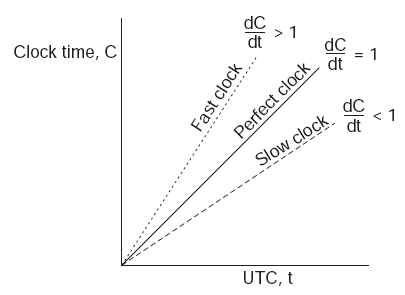
\includegraphics[scale=0.4]{./figures/phys-clock.png}
    \end{figure}
    \begin{block}{Goal}
        Never let 2 clocks in any system differ by more than $\delta$ time units => \\
        Syncronize at least every $\delta/(2r)$ seconds.
    \end{block}
\end{frame}

\begin{frame}
    \frametitle{Physical Clocks}
    Clock Syncronization Principle
    \begin{block}{Principle I}
        Every machine asks a timer server for the accurate time at least every $\delta/(2r)$ seconds(Network Time Protocol).
    \end{block}
    \begin{block}{Principle II}
        Let the server scan all machines periodically, calculate an average, and inform each machine how it should adjust its time relative to its present time.
    \end{block}
\end{frame}

\begin{frame}
    \frametitle{Logic Clock}
    \begin{block}{Why not physical clock?}
        \begin{itemize}
            \item Nodes may differ on real time at ms level using NTP.
            \item It's not necessary. If two processes do not interact, it is not necessary that their clocks be syncronized because the lack of synchronization would not be observable and thus could not cause problem.
            \item What usually matters is not that all processes agree on exactly what time it is, but rather that they agree on the order in which events occur.
        \end{itemize}
    \end{block}
\end{frame}

\begin{frame}
    \frametitle{Partial Order}
    \begin{block}{Definition}
        Orders are special binary relations. Suppose that P is a set and that $\le$ is a relation on P. Then $\le$ is a \alert{partial order} if it is \alert{reflexive}, \alert{antisymmetric}, and \alert{transitive}. i.e., for all a, b and c in P, we have that: \\
        \begin{gather}
            a \le a (reflexive) \\
            \mbox{ if } a \le b \mbox{ and } b \le a \mbox{ then } a = b (antisymmetric) \\
            \mbox{ if } a \le b \mbox{ and } b \le c \mbox{ then } a \le c (transitive)
        \end{gather}
    \end{block}
\end{frame}

\begin{frame}
    \frametitle{Happens Before}
    \begin{block}{The happens before \to relation}
        \begin{itemize}
            \item $a \to b$, if a and b are events in the same process and a occurred before b.
            \item $a \to b$, if a is the event of sending a message m in a process and b is the event of receipt of the same message by another process
            \item if $a \to b$ and $b \to c$, then $a \to c$ (transitive).
            \item concurrent: $ a || b$ if $!(a \to b)$ and $!(b \to a)$.
            \item for any 2 events in a system, either $a \to b$ or $b \to a$ or $a || b$.
        \end{itemize}
    \end{block}
    \begin{figure}
        \centering
        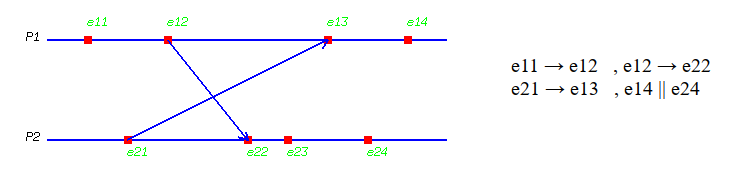
\includegraphics[scale=0.28]{./figures/lamport.png}
    \end{figure}
\end{frame}

\begin{frame}
    \frametitle{Lamport Clock}
    \begin{figure}
        \centering
        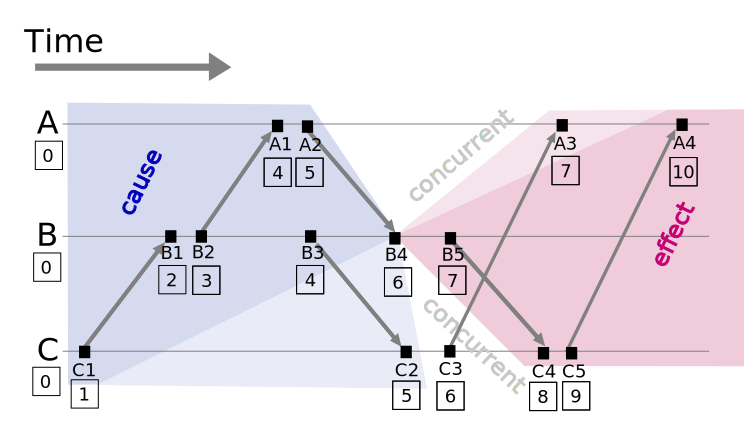
\includegraphics[scale=0.3]{./figures/Lamport-Clock}
    \end{figure}
    \begin{itemize}
        \item 每个事件对应一个Lamport时间戳,初始值为0
        \item 如果为节点内发生事件,时间戳加1
        \item 如果为发送事件,时间戳加1并在消息中带上该时间戳
        \item 如果为接收事件,时间戳=Max(本地时间戳,消息中的时间戳)+1
    \end{itemize}
\end{frame}

\begin{frame}
    \frametitle{Positioning of Lamport Clock in DS}
    \begin{figure}
        \centering
        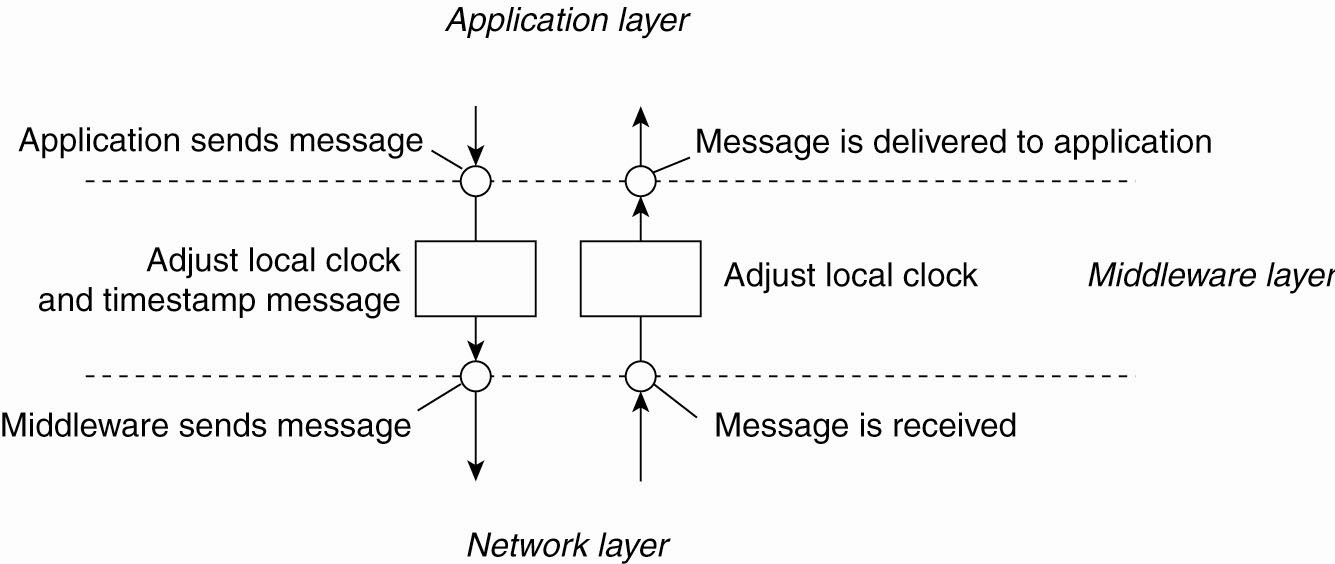
\includegraphics[scale=0.32]{./figures/lamport-position.jpg}
    \end{figure}
\end{frame}

\begin{frame}
    \frametitle{Lamport Clock}
    \begin{block}{Limitation of Lamport-Clock}
        $C_i(a)$ -- timestamp of event a at $P_i$ \\
        if $a \to b$, then $C(a) < C(b)$ \\
        but $C(a) < C(b)$ does not necessarily imply $a \to b$
    \end{block}
    \begin{itemize}
        \item Vector Clock overcome the shortcoming of Lamport Clock
        \item Goal
            \begin{itemize}
                \item Want ordering that matches causality.
                \item $C(a) < C(b)$ if and only if $a \to b$.
            \end{itemize}
        \item Method: label each event by vector V(e) [c1, c2, \ldots, cn].
    \end{itemize}
\end{frame}

\begin{frame}
    \frametitle{Vector Clock}
    \begin{figure}
        \centering
        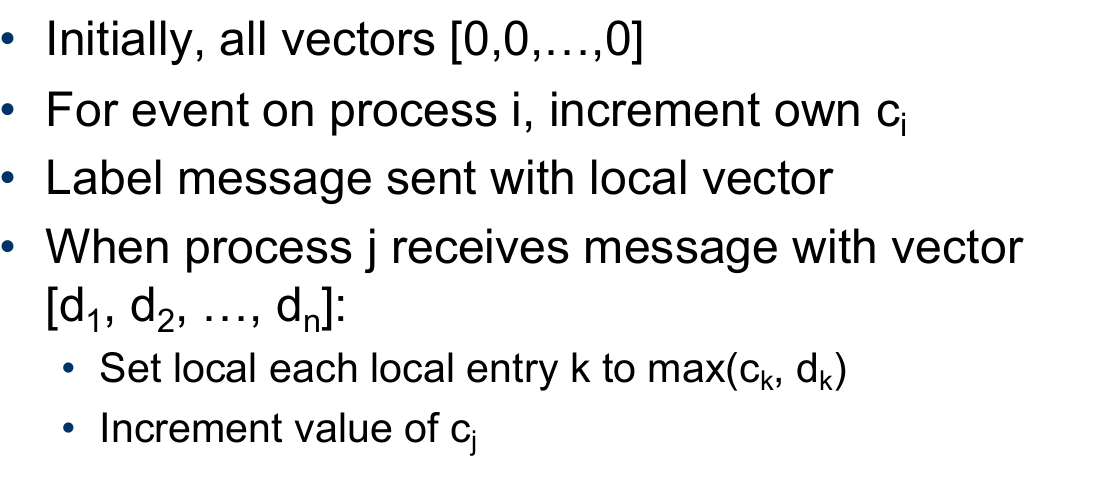
\includegraphics[scale=0.3]{./figures/vector-clock1.png}
    \end{figure}
\end{frame}

\begin{frame}
    \frametitle{Vector Clock}
    \begin{figure}
        \centering
        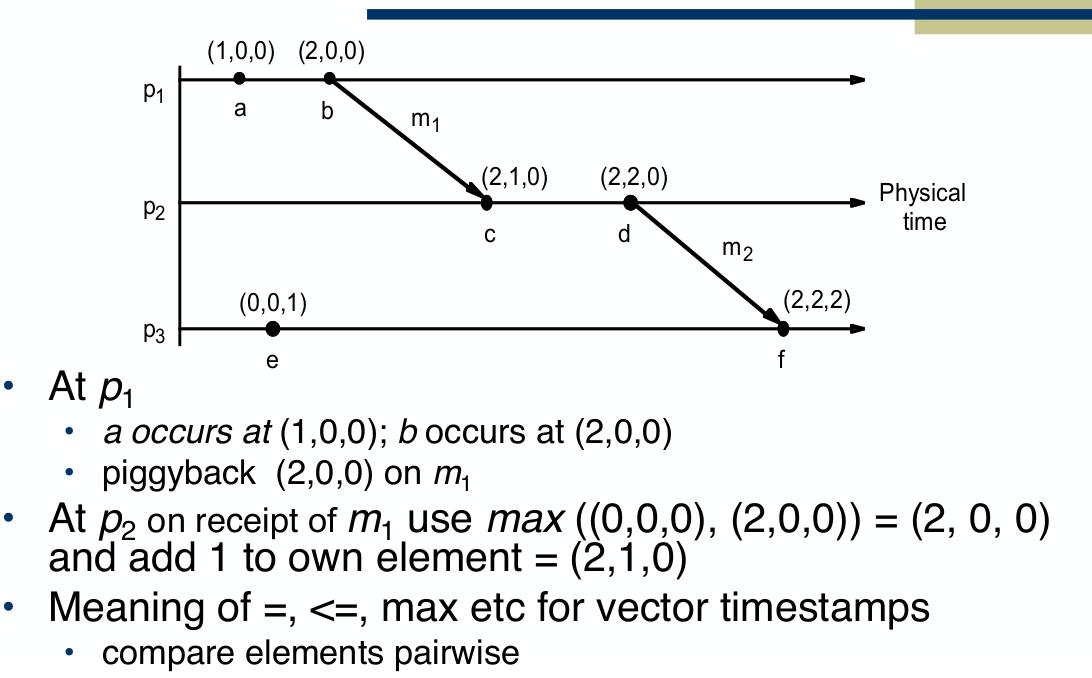
\includegraphics[scale=0.3]{./figures/vector-clock2.png}
    \end{figure}
\end{frame}

\begin{frame}
    \frametitle{Vector Clock}
    \begin{figure}
        \centering
        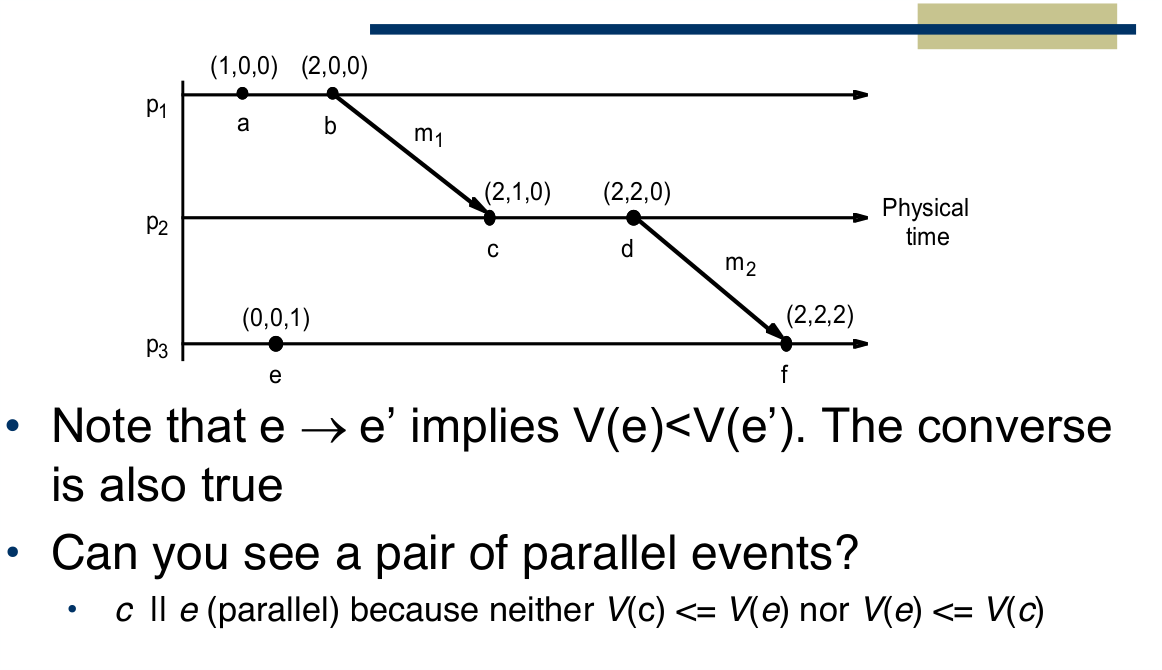
\includegraphics[scale=0.3]{./figures/vector-clock3.png}
    \end{figure}
\end{frame}

\begin{frame}
    \frametitle{Review}
    \begin{itemize}
        \item Clock Syncronization
            \begin{itemize}
                \item Rely on a time-stamped network messages
                \item Estimate delay for message transmission
                \item Can synchronize to UTC or to local source
                \item Clocks never exactly syncronized
                \item Often inadequate for distributed system
            \end{itemize}
        \item Logical Clocks
            \begin{itemize}
                \item Encode causality relationship
                \item Lamport clocks provide only one-way encoding
                \item Vector clocks provide exact causality information
            \end{itemize}
    \end{itemize}
\end{frame}

\begin{frame}
    \frametitle{Election Algorithms}
A Centralized Algorithm
\begin{itemize}
    \item One process is elected as the coordinator.
    \item Whenever a process wants to access a shared-resource, it sends request to the coordinator to ask for permission.
    \item Coordinator may queue requests.
\end{itemize}
\begin{figure}
    \centering
    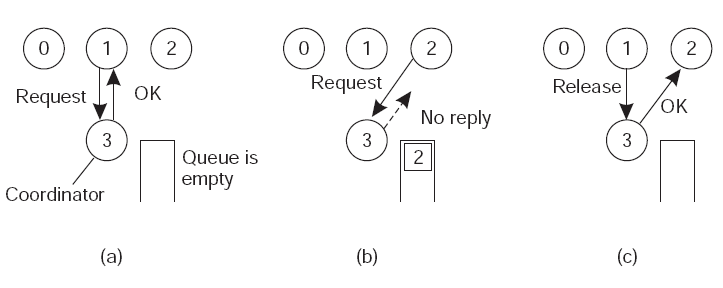
\includegraphics[scale=0.4]{./figures/mutual-exclusion.png}
\end{figure}

\end{frame}

\begin{frame}
    \frametitle{Election Algorithm}
\begin{block}{Principle}
    An algorithm requires that some process acts as a coordinator. The question is how to select this special process dynamically.
\end{block}

\end{frame}

\begin{frame}
    \frametitle{Election by bullying}
\begin{block}{Principle}
    Each process has an associated priority(weight). The process with the highest priority should always be elected as the coordinator.
\end{block}

\begin{block}{Issue: How do we find the heaviest process?}
    \begin{itemize}
        \item Any process can just start an election by sending an election message to all other processes with higher numbers.
        \item If a process $P_{heavy}$ receives an election message from a lighter process $P_{light}$, it sends a take-over message to $P_{light}$. $P_{light}$ is out of the race.
        \item If a process doesn't get a take-over message back, it wins, and sends a victory message to all other processes.
    \end{itemize}
\end{block}

\end{frame}

\begin{frame}
    \frametitle{Election by bullying}
    \begin{figure}
        \centering
        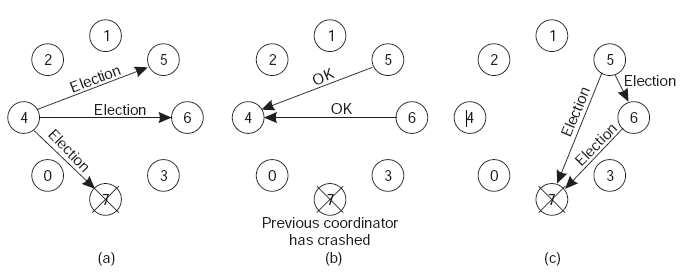
\includegraphics[scale=0.4]{./figures/bully.png}
        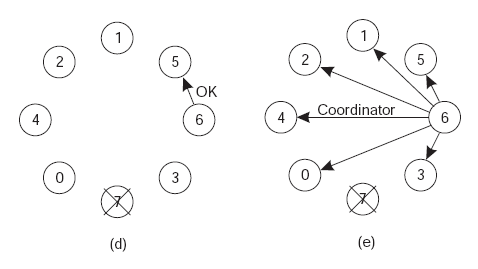
\includegraphics[scale=0.4]{./figures/bully2.png}
    \end{figure}
(a) Process 4 holds an election. \\
(b) Processes 5 and 6 responded, telling 4 to stop. \\
(c) Now 5 and 6 hold an election. \\
(d) Process 6 tells 5 to stop. \\
(e) Process 6 wins an tells everyone.
\end{frame}

\begin{frame}
    \frametitle{Election by bullying}
    \begin{block}{Issue}
    Suppose crashed nodes comes back online:
    \begin{itemize}
        \item Sends a new election message to higher numbered processes.
        \item Repeat until only one process left standing.
        \item Announces victory by sending message saying that it is coordinator(if not already coordinator)
        \item Existing(lower numbered) coordinator yields.
    \end{itemize}
    \end{block}
    Hence the term 'bully'
\end{frame}

\begin{frame}
    \frametitle{Election in a ring}
    \begin{block}{Principle}
        Process priority is obtained by organizing process into a (logical) ring. Process with the highest priority should be elected as coordinator.
    \end{block}

    \begin{itemize}
        \item Any process can start an election by sending an election message to its successor. If a successor is down, the message is passed on to the next successor.
        \item If a message is passed on, the sender adds itself to the list. When it gets back to the initiator, everyone had a chance to make its presence known.
        \item The initiator sends a coordinator message around the ring containing a list of all living processes. The one with the highest priority is elected as coordinator.
    \end{itemize}
\end{frame}

